\section{Projeto de Pontes de Madeiras}\label{sec:ponte_madeira}

As pontes de madeira, uma das formas mais antigas de estrutura de travessia, evoluíram significativamente em sua concepção e aplicação.
Atualmente, podem ser classificadas em diversos tipos estruturais, cada um com suas particularidades, vantagens e contextos de aplicação adequados.
O objetivo desta seção é apresentar alguns modelos de pontes de madeira e particularidades de dimensionamento.

\subsection{Tipologias de pontes de madeiras}

As tipologias de pontes de madeira são as mais variadas possíveis e, neste trabalho, serão apresentados apenas modelos de pontes de madeira em viga.
Segundo a classificação proposta por \textcite{ritter1990}, as superestruturas em viga podem ser subdivididas nos seguintes tipos:
\begin{itemize}
    \item vigas de toras roliças (\textit{log beams});
    \item vigas de madeira serrada (\textit{sawn lumber beams});
    \item vigas de madeira laminada colada (\textit{glued-laminated timber beams} -- MLC);
    \item vigas de madeira laminada colada de lâminas paralelas (\textit{laminated veneer lumber beams} -- LVL).
\end{itemize}

A Figura \ref{fig:pontenat} apresenta exemplos de pontes de madeira que são comumente encontradas
em regiões de estradas vicinais do Brasil. A ponte exemplificada consiste em \tofill{descrever o sistema 
construtivo observado na figura: espécie de madeira, número de longarinas, tipo de tabuleiro e conexões}.

\begin{figure}[htpb!]
    \centering
    \caption{Ponte de madeira nativa roliças.}
    \label{fig:pontenat}
    
  % primeira imagem
    \begin{minipage}[t]{0.45\textwidth}
        \centering
        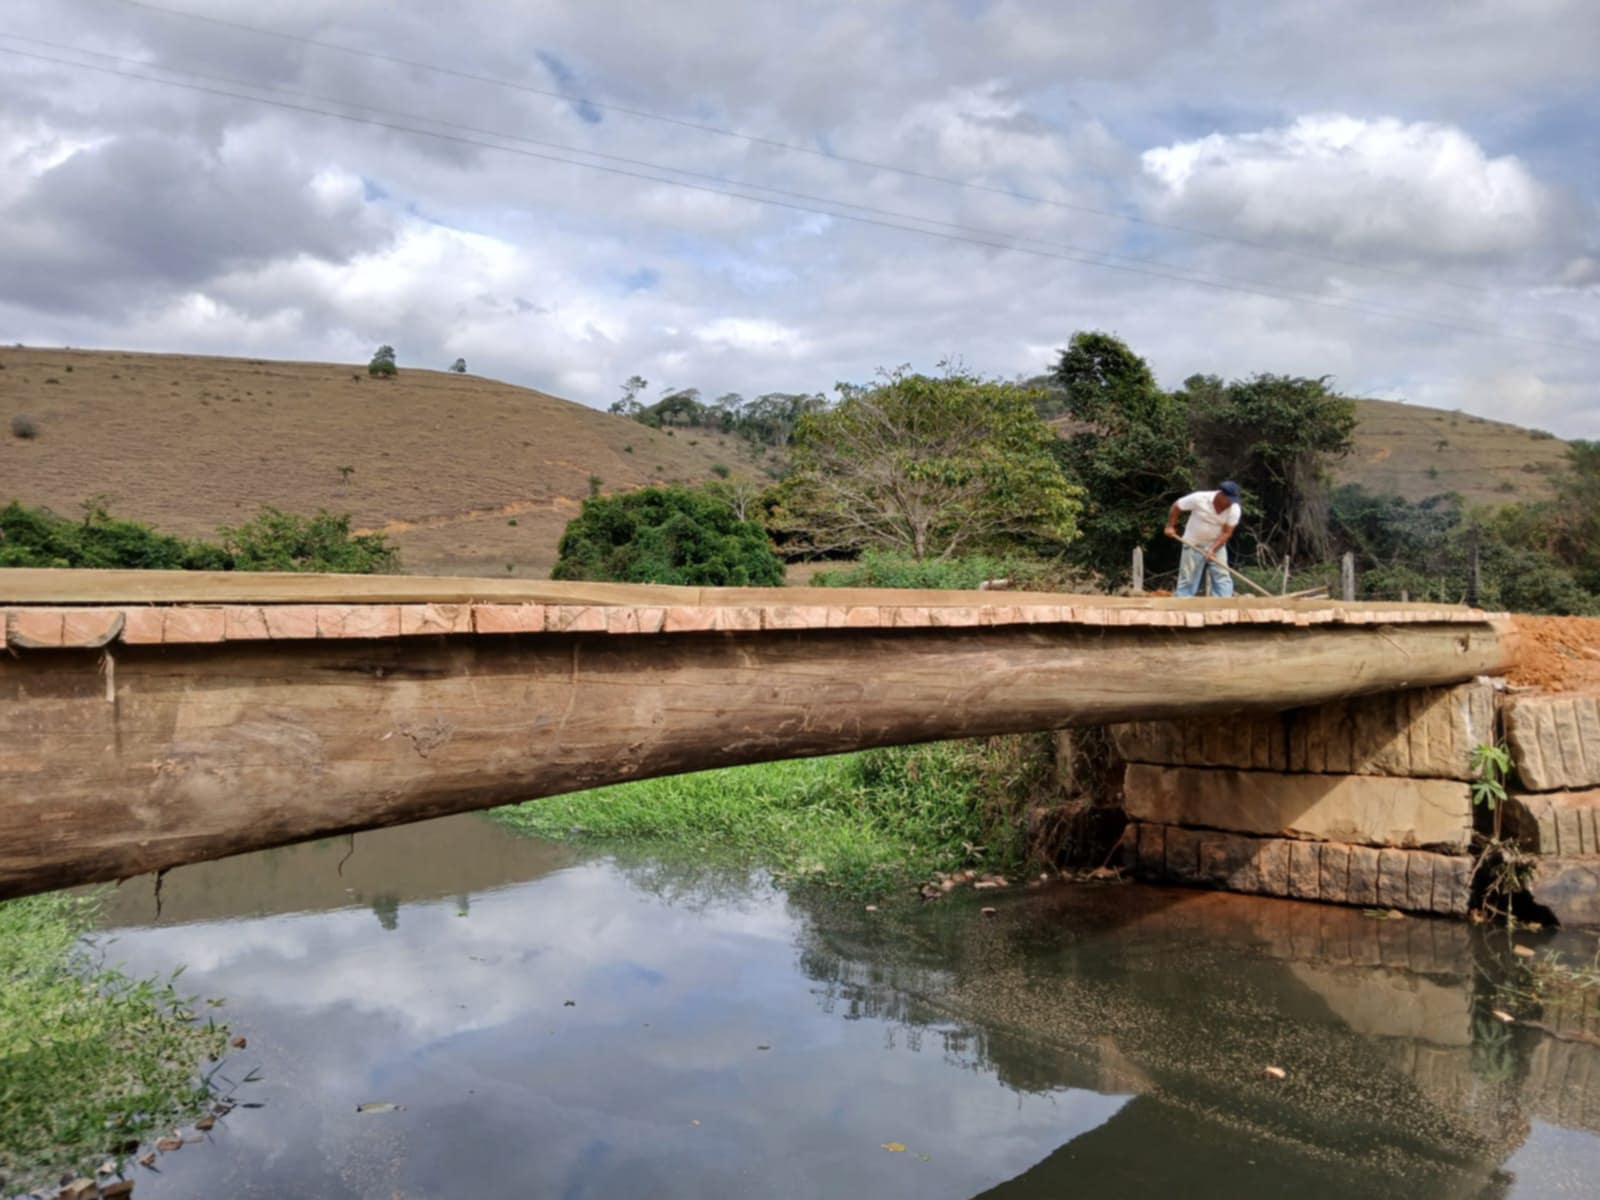
\includegraphics[width=\textwidth]{figuras/pontenativa.jpg}
    \end{minipage}
     % segunda imagem
    \begin{minipage}[t]{0.45\textwidth}
        \centering
        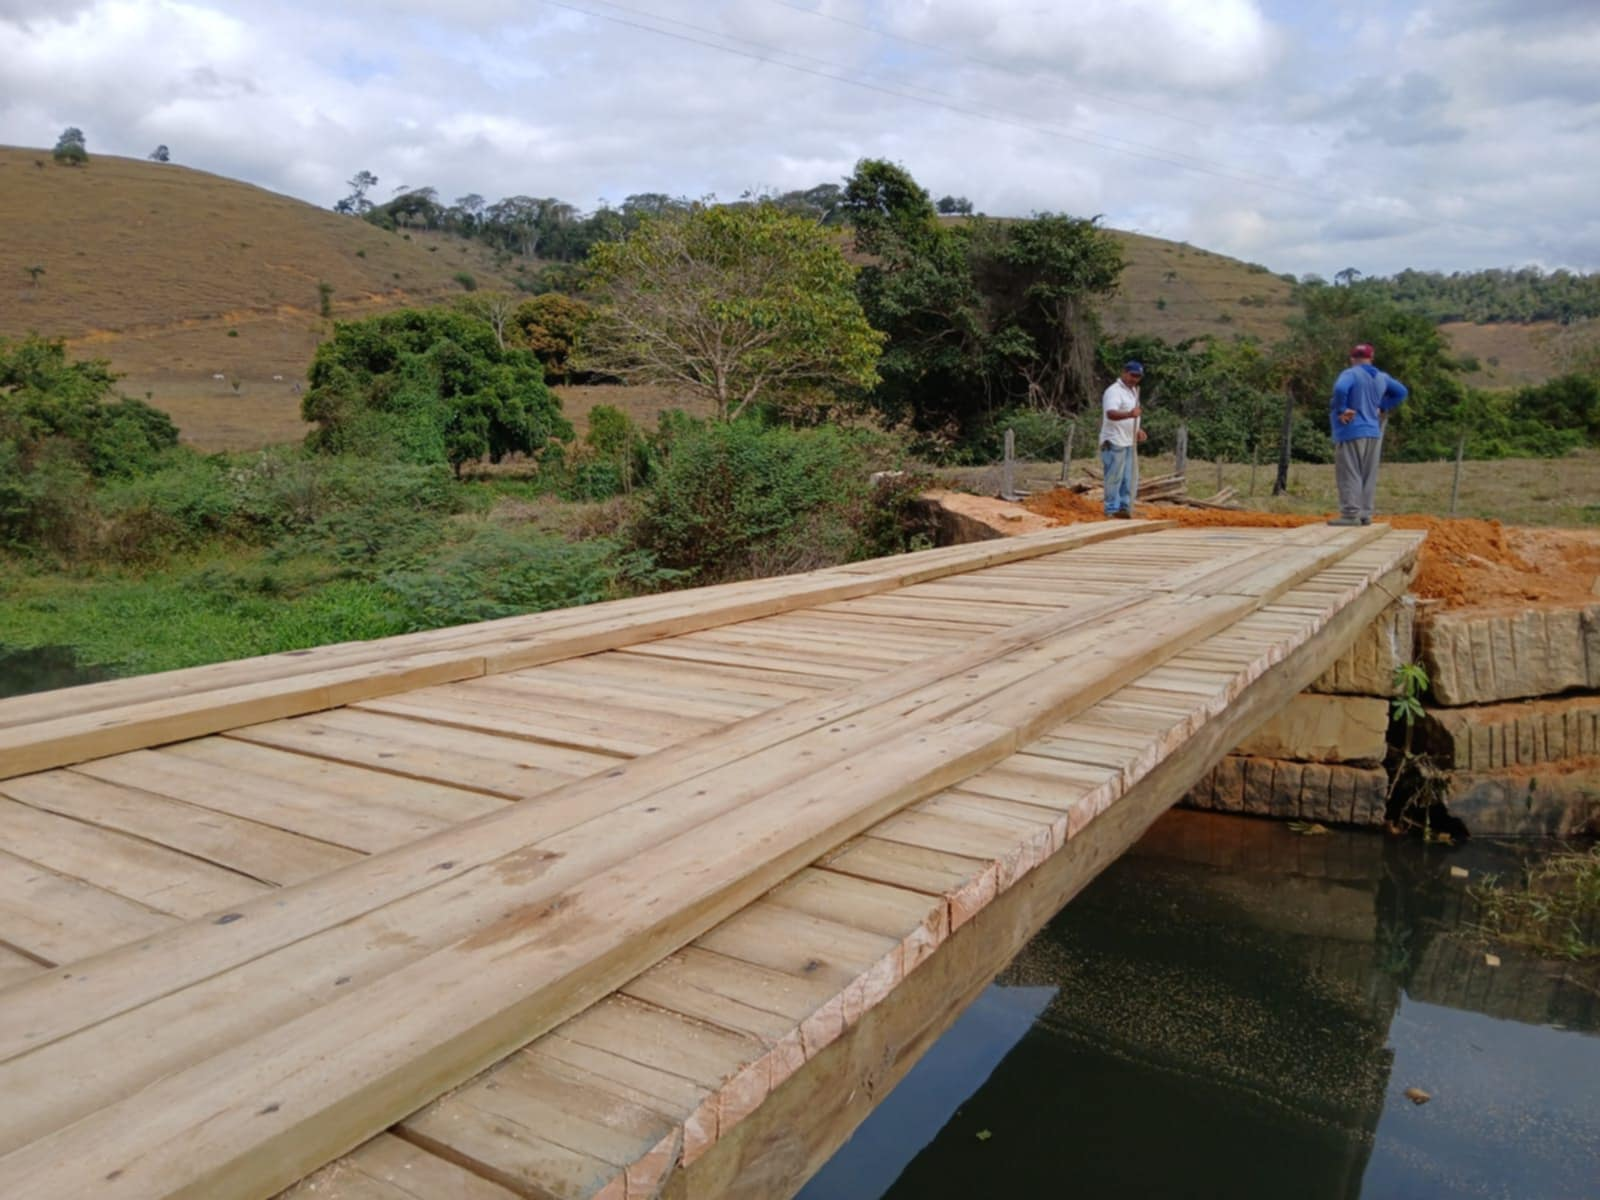
\includegraphics[width=\textwidth]{figuras/pontenativa2.jpg}
    \end{minipage}

    \vspace{0.2cm}
    \small Fonte: \parencite{gazeta2025ponte}.
\end{figure}

Segundo \textcite{ritter1990}, a extensão do vão, em pontes de toras roliças, depende da espécie, diâmetro e
comprimento das árvores disponíveis.
Vãos frequentes variam entre 6 e 18 metros, mas há exemplares documentados que se aproximam dos 30 metros, capazes de suportar
veículos com carga total superior a 100 toneladas.

\subsection{Diâmetro das toras roliças}

\begin{fillblock}
Descrever o critério de determinação do diâmetro equivalente da tora roliça (por exemplo, diâmetro na seção correspondente a 1/3 do comprimento da peça a partir da extremidade de maior diâmetro). Incluir figura esquemática com o diâmetro mínimo, médio e equivalente ao longo do comprimento da peça (arquivo a salvar em \texttt{figuras/}).
\end{fillblock}

\subsection{Carga do trem tipo}\label{sec:trem_tipo}

As cargas delimitadas nas pontes brasileiras são definidas pela \textcite{nbr7188}, que estabelece 
os requisitos para o projeto de pontes rodoviárias.

A norma apresenta dois modelos de trem-tipo para uso: o TB-450 e o TB-240. Porém, por se tratar de estradas vicinais,
serão contemplados apenas os detalhes do TB-240.
Esse trem-tipo é caracterizado por um veículo de 240 kN de peso total, constituído por seis rodas e três eixos.
Cada eixo do veículo aplica uma carga de 40 kN, com espaçamentos de 1,5 m entre os eixos.
A área de ocupação do veículo deve ser de 18,0 m², complementada por uma carga
uniformemente distribuída de 4,0 kN/m² em seu entorno (multidão), conforme a Figura \ref{fig:trem}.

\begin{figure}[htpb!]
    \centering
    \caption{Configuração trem de tipo.}
    \label{fig:trem}
    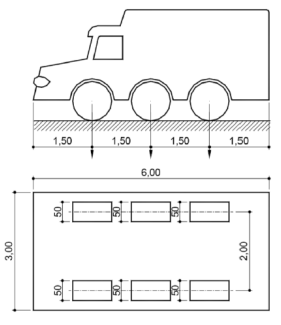
\includegraphics[width=0.4\textwidth]{figuras/trem1.png}\\    
    \vspace{0.2cm}
    \centering \small Fonte: \parencite{nbr7188}
\end{figure}

\subsection{Propriedades da Madeira}

\subsubsection{Estrutura da madeira}

\begin{fillblock}
Descrever brevemente a anisotropia da madeira (direções longitudinal, radial e tangencial) e sua relação com as propriedades mecânicas empregadas nas verificações desta seção, em especial a resistência à compressão e a resistência à flexão paralelas às fibras.
\end{fillblock}

\subsubsection{Ponderadores para propriedades mecânicas}

Para a realização dessas verificações, a \textcite{NBR7190-1:2022} estabelece parâmetros de resistência ($f$) e de módulo de elasticidade ($E$), bem como classes de resistência para madeiras dos grupos das Coníferas e das Folhosas, sob condição padrão de referência, isto é, teor de umidade ($U$) igual a 12\%.

Conforme o item 5.6.1 da \textcite{NBR7190-1:2022}, esses valores de referência correspondem à classe de umidade 1, definida pelo teor de umidade de equilíbrio de 12\%.
Quando a caracterização das propriedades de resistência e de rigidez de um lote de madeira é realizada com teores de umidade distintos, no intervalo entre 10\% e 25\%, os resultados devem ser corrigidos para a umidade-padrão de 12\% por meio das Equações~\eqref{eq:corr_resist} e~\eqref{eq:corr_rigidez}.

\begin{equation}
f_{12} = f_U \left[1 + \frac{3\,(U - 12)}{100}\right]
\label{eq:corr_resist}
\end{equation}

\begin{equation}
E_{12} = E_U \left[1 + \frac{2\,(U - 12)}{100}\right]
\label{eq:corr_rigidez}
\end{equation}

sendo $f_U$ e $E_U$ os valores de resistência e de rigidez obtidos no ensaio para o teor de umidade $U$ (em \%), e $f_{12}$ e $E_{12}$ os valores correspondentes já corrigidos para a condição-padrão de referência.

\begin{fillblock}
A \textcite{NBR7190-1:2022} também estabelece uma correção análoga para a massa específica aparente ($\rho_{ap}$) em função do teor de umidade. Transcrever aqui a equação de correção de $\rho_{ap}$ apresentada na norma (item imediatamente seguinte ao 5.6.1), indicando o item correspondente. Observação: as densidades das classes de resistência empregadas pela plataforma (Tabela de classes de resistência, coluna $\rho_{12\%}$) já são tabeladas na condição-padrão de 12\%, de modo que essa correção só é necessária caso se utilizem valores de densidade obtidos diretamente em ensaio, com teor de umidade diferente de 12\%.
\end{fillblock}

O método dos estados limites baseia-se na premissa de majoração dos esforços e minoração das resistências ($f$) e do módulo de elasticidade ($E$).
Os coeficientes de minoração têm por objetivo compensar as incertezas associadas à resistência característica, bem como os efeitos adversos das imperfeições geométricas.
A \textcite{NBR7190-1:2022} propõe essa minoração por meio da utilização dos coeficientes de modificação ($k_{\mathrm{mod}}$) e do coeficiente de ponderação da resistência ($\gamma_w$), conforme apresentado na equação \ref{eq:2.099}.

\begin{equation}
    X_d = \frac{k_{\mathrm{mod}} \cdot X_k}{\gamma_w}
\label{eq:2.099}
\end{equation}
Onde:
\begin{itemize}
    \item $X_k$ é o valor característico da resistência da madeira;
    \item $k_{\mathrm{mod}}$ é o coeficiente de modificação da madeira;
    \item o coeficiente de ponderação da resistência ($\gamma_w$) assume o valor de 1{,}4 para tensões normais e 1{,}8 para tensões de cisalhamento.
\end{itemize}

O coeficiente de modificação ($k_{\mathrm{mod}}$) altera os valores característicos das propriedades de resistência da madeira em função da classe de carregamento da estrutura e da classe de umidade admitida, sendo calculado conforme a Equação \ref{eq:2.99}.

\begin{equation}
k_{\mathrm{mod}} = k_{\mathrm{mod},1} \cdot k_{\mathrm{mod},2}
\label{eq:2.99}
\end{equation}

O primeiro fator, $k_{\mathrm{mod},1}$, está associado à classe de carregamento, sendo definido em função da duração acumulada da ação variável principal da combinação e do tipo de madeira empregado, de acordo com o item 5.8.4.1 da norma. Os valores correspondentes às diferentes classes de carregamento e aos grupos de materiais são apresentados na Tabela \ref{tab:kmod1.q}.

\begin{table}[htpb!]
\centering
\caption{Classes de carregamento e fatores de modificação (\textit{$k_{mod,1}$}).}
\label{tab:kmod1.q}
\footnotesize
\begin{tabular}{
>{\centering\arraybackslash}m{2.8cm}
>{\centering\arraybackslash}m{2.2cm}
>{\centering\arraybackslash}m{3.8cm}
>{\centering\arraybackslash}m{4.6cm}
>{\centering\arraybackslash}m{1.8cm}
}
\hline
\multirow{4}{*}{\shortstack{\textbf{Classes de} \\ \textbf{carregamento}}} &
\multicolumn{2}{c}{\textbf{Ação variável principal da combinação}} &
\multirow{4}{*}{\shortstack{\textbf{Tipos de madeira}}} &
\multirow{4}{*}{\shortstack{\textbf{Madeira} \\ \textbf{Recomposta}}}\\
\cline{2-3}
& \textbf{Duração acumulada} &
\textbf{Ordem de grandeza da duração acumulada da ação característica} &
& \\
\hline
Permanente &
Permanente &
Mais de dez anos &
Madeira serrada \newline
Madeira roliça \newline
Madeira laminada colada (MLC) \newline
Madeira laminada colada cruzada (MLCC) \newline
Madeira laminada colada (LVL) &
0,30 \\
\hline
Longa duração &
Longa duração &
Seis meses a dez anos &
0,70 &
0,45 \\
%\hline
Média duração &
Média duração &
Uma semana a seis meses &
0,80 &
0,65 \\
%\hline
Curta duração &
Curta duração &
Menos de uma semana &
0,90 &
0,90 \\
%\hline
Instantânea &
Instantânea &
Muito curta &
1,10 &
1,10 \\
\hline
\end{tabular}

\vspace{0.3cm}
\centering
\small Fonte: Adaptado de ABNT NBR 7190:2023.
\end{table}


O segundo fator, $k_{\mathrm{mod},2}$, está relacionado à classe de umidade à qual o elemento estrutural está submetido, bem como ao tipo de material utilizado, conforme especificado no item 5.8.4.2 da \textcite{NBR7190-1:2022}.
Os valores normativos desse coeficiente, diferenciados entre madeiras maciças, produtos engenheirados e madeiras recompostas, encontram-se sistematizados na Tabela \ref{tab:kmod2.2}.


\begin{table}[htpb!]
\centering
\caption{Valores de (\textit{$k_{mod,2}$}).}
\label{tab:kmod2.2}
\footnotesize
\begin{tabular}{
>{\centering\arraybackslash}p{3cm} 
>{\centering\arraybackslash}p{6cm} 
>{\centering\arraybackslash}p{2cm}
}
\hline
\multirow{2}{*}{\textbf{Classes de umidade}} & 
\multirow{2}{*}{\textbf{Tipos de madeira}} & 
\textbf{Madeira recomposta} \\
\hline
 &  Madeira serrada \newline
Madeira roliça \newline
Madeira laminada colada (MLC) \newline
Madeira laminada colada cruzada (MLCC) \newline
Madeira laminada colada (LVL) & \\
\hline
(1) & 1,00 & 1,00 \\
%\hline
(2) & 0,90 & 0,95 \\
%\hline
(3) & 0,80 & 0,93 \\
%\hline
(4) & 0,70\textsuperscript{a} & 0,90 \\
\hline
\end{tabular}

\vspace{0.2cm}
\centering
\footnotesize\textsuperscript{a}\,Não é permitido o uso do MLCC para classe de umidade (4).\\
\small Fonte: Adaptado de ABNT NBR 7190:2023.
\end{table}

\subsection{Flecha limite}\label{sec:flecha_limite}

\subsubsection{Fluência}

Além dos valores médios do módulo de elasticidade, a \textcite{NBR7190-1:2022} estabelece que, nas verificações em que a rigidez ao longo do tempo é relevante, deve ser considerado o valor efetivo do módulo de elasticidade, $E_{0,\mathrm{ef}}$, conforme a Equação \ref{eq:2.558}, empregado no cálculo das flechas finais $\delta_{\mathrm{fin},G_i,k}$ e $\delta_{\mathrm{fin},Q_j,k}$, associadas respectivamente às ações permanentes e variáveis, conforme as Equações \ref{eq:flecha_fin_G} e \ref{eq:flecha_fin_Q}.

\begin{equation}
E_{0,\mathrm{ef}} = k_{\mathrm{mod},1} \cdot k_{\mathrm{mod},2} \cdot E_{0,\mathrm{med}}
\label{eq:2.558}
\end{equation}

\begin{equation}
\delta_{\mathrm{fin},G_i,k}
=
\delta_{\mathrm{inst},G_i,k}
+ \delta_{\mathrm{creep}}
=
\delta_{\mathrm{inst},G_i,k} \cdot (1 + \varphi)
\label{eq:flecha_fin_G}
\end{equation}

\begin{equation}
\delta_{\mathrm{fin},Q_j,k}
=
\delta_{\mathrm{inst},Q_j,k}
+ \delta_{\mathrm{creep}}
=
\delta_{\mathrm{inst},Q_j,k} \cdot \psi_{2} \cdot (1 + \varphi)
\label{eq:flecha_fin_Q}
\end{equation}

Segundo a \textcite{NBR7190-1:2022}, ``a madeira possui características distintas de outros materiais de construção, como, por exemplo, a significativa deformação ao longo do tempo (fluência)''.
Em razão dessa condição, torna-se necessária a aplicação do coeficiente de fluência ($\varphi$) na estimativa dos deslocamentos finais ou efetivos, conforme as Equações \ref{eq:flecha_fin_G} e \ref{eq:flecha_fin_Q}.
Esse coeficiente é definido em função do material e da classe de umidade à qual o sistema estrutural está exposto.
Classes de umidade mais elevadas resultam em flechas mais acentuadas, conforme evidenciado pelos valores do coeficiente de fluência apresentados na Tabela \ref{tab:fluencia}.

\begin{table}[htpb!]
\centering
\caption{Coeficiente de fluência ($\varphi$).}
\label{tab:fluencia}
\footnotesize
\begin{tabular}{
>{\centering\arraybackslash}m{6.0cm}
>{\centering\arraybackslash}m{2.5cm}
>{\centering\arraybackslash}m{2.5cm}
>{\centering\arraybackslash}m{2.5cm}
}
\hline
\multirow{2}{*}{\textbf{Materiais}} &
\multicolumn{3}{c}{\textbf{Classe de umidade}} \\
\cline{2-4}
& \textbf{(1)} & \textbf{(2 e 3)} & \textbf{(4)} \\
\hline
Madeira serrada, MLC, MLCC, LVL e roliça
& 0,6 & 0,8 & 2,0\textsuperscript{a} \\
\hline
Compensado estrutural
& 0,8 & 1,0 & 2,5 \\
\hline
OSB estrutural
& 1,5 & 2,25 & -- \\
\hline
\end{tabular}

\vspace{0.3cm}
\small\textsuperscript{a} Não é permitido o uso de MLCC para a classe de umidade 4.\\
\small Fonte: Adaptado de \textcite{NBR7190-1:2022}.
\end{table}

\subsubsection{Limites normativos de flecha}

Na verificação do Estado Limite de Serviço (ELS), a \textcite{NBR7190-1:2022} estabelece valores limites para as flechas, considerando-se a flecha instantânea ($\delta_{\mathrm{inst}}$) e a flecha final ($\delta_{\mathrm{fin}}$).
Esses valores limites dependem da configuração estática da estrutura e encontram-se apresentados na Tabela \ref{tab:flechas_limites}.

\begin{table}[htpb!]
\centering
\caption{Flechas limites para elementos correntes fletidos.}
\label{tab:flechas_limites}
\footnotesize
\begin{tabular}{
>{\centering\arraybackslash}m{5.0cm}
>{\centering\arraybackslash}m{3.0cm}
>{\centering\arraybackslash}m{3.0cm}
}
\hline
\textbf{Tipo} & $\boldsymbol{\delta_{inst}}$ & $\boldsymbol{\delta_{fin}}$ \\
\hline
Vigas biapoiadas ou contínuas
& L/300 a L/500
& L/150 a L/300 \\
\hline
Vigas em balanço
& L/150 a L/250
& L/75 a L/150 \\
\hline
\end{tabular}

\vspace{0.3cm}
\small Fonte: Adaptado da ABNT NBR 7190-1 (2022) .
\end{table}

Logo, o dimensionamento de sistemas estruturais em madeira deve atender a esses requisitos normativos.

\subsection{Projeto da ponte}\label{sec:projeto_ponte}

O sistema estrutural considerado é composto por um tabuleiro de pranchas retangulares de madeira, de largura $b_w$ e altura $h$, apoiado continuamente sobre longarinas circulares roliças de diâmetro $d$, tratadas analiticamente como vigas biapoiadas de vão $L$.
As etapas de verificação seguem a sequência: determinação dos esforços solicitantes, verificação à flexão e ao cisalhamento da longarina, verificação da flecha e, por fim, verificação à flexão do tabuleiro.
O procedimento de cálculo apresentado nesta seção segue os critérios normativos da ABNT NBR 7190-1 e o roteiro de dimensionamento do Manual de Projeto e Construção de Pontes de Madeira \parencite{CALIL2006}.

\subsubsection{Esforços}

Para a longarina circular maciça, a área, o momento de inércia, o módulo resistente e o raio de giração são obtidos pelas Equações~\eqref{eq:areacirc} a~\eqref{eq:rcirc}.

\begin{equation}
A = \frac{\pi d^2}{4}
\label{eq:areacirc}
\end{equation}

\begin{equation}
I_x = I_y = \frac{\pi d^4}{64}
\label{eq:icirc}
\end{equation}

\begin{equation}
W_x = W_y = \frac{I_x}{d/2}
\label{eq:wcirc}
\end{equation}

\begin{equation}
r_x = r_y = \sqrt{\frac{I_x}{A}}
\label{eq:rcirc}
\end{equation}

Para as pranchas retangulares do tabuleiro, a área e o momento de inércia em relação ao eixo de flexão são dados pelas Equações~\eqref{eq:arearet} e~\eqref{eq:iret}.

\begin{equation}
A = b_w\,h
\label{eq:arearet}
\end{equation}

\begin{equation}
I_x = \frac{b_w\,h^3}{12}
\label{eq:iret}
\end{equation}

As ações permanentes correspondem ao peso próprio das longarinas, do tabuleiro e demais elementos, obtidas em função da geometria e do peso específico $\gamma$, conforme a Equação~\eqref{eq:permanente}.

\begin{equation}
G = \gamma \cdot A
\label{eq:permanente}
\end{equation}

A carga móvel considerada é o trem-tipo TB-240 apresentado na Seção~\ref{sec:trem_tipo}, representado por um veículo de três eixos e seis rodas, cada roda transmitindo uma carga $P$ de 40~kN, além da carga de multidão uniformemente distribuída $q$.
Os efeitos dinâmicos são incorporados pelo coeficiente de impacto vertical ($CIV$), determinado pelas Equações~\eqref{eq:civ1} e~\eqref{eq:civ2} conforme o item \tofill{7.2.3} da \textcite{nbr7188}, sendo $LIV$ o comprimento característico da estrutura \tofill{(conferir, no item da norma, se corresponde ao vão da longarina ou ao comprimento total da ponte)}.

\begin{equation}
CIV = 1{,}35 \qquad \text{para } L \leq 10{,}0\ \text{m}
\label{eq:civ1}
\end{equation}

\begin{equation}
CIV = 1 + 1{,}06\left(\frac{20}{LIV + 50}\right), \qquad \text{para } 10{,}0 < L \leq 200{,}0\ \text{m}
\label{eq:civ2}
\end{equation}

A plataforma aplica ainda um fator de atenuação sobre o excedente do coeficiente de impacto em relação à unidade, de modo que apenas 75\% desse excedente amplifique de fato os esforços variáveis, conforme a Equação~\eqref{eq:civaux}.
O fator resultante, $aux_{ci}$, multiplica diretamente os esforços solicitantes de origem variável.

\begin{equation}
aux_{ci} = 1 + 0{,}75\,(CIV - 1)
\label{eq:civaux}
\end{equation}

O momento fletor e o esforço cortante máximos devidos à carga permanente, assim como a flecha estática correspondente, são quantificados pelas premissas clássicas de estática para vigas biapoiadas, conforme as Equações~\eqref{eq:mgk} e~\eqref{eq:qgk}.
Para a carga variável, adota-se o posicionamento mais desfavorável das rodas do trem-tipo sobre o vão, resultando no momento fletor $M_{qk}$ das Equações~\eqref{eq:mqk30} e~\eqref{eq:mqk45}, dependente da extensão do vão, e na força cortante $Q_{qk}$ da Equação~\eqref{eq:qqk}, sendo $a$ a distância entre o apoio e a roda mais próxima, com as grandezas auxiliares $c$ e $e$ definidas pelas Equações~\eqref{eq:cmomento} e~\eqref{eq:ecortante}.

\begin{equation}
M_{gk} = \frac{g\,L^2}{8}
\label{eq:mgk}
\end{equation}

\begin{equation}
Q_{gk} = \frac{g\,L}{2}
\label{eq:qgk}
\end{equation}

\begin{equation}
c = \frac{L - 4a}{2}, \qquad \text{para } L > 6\,\text{m}
\label{eq:cmomento}
\end{equation}

\begin{equation}
M_{qk} = \frac{3\,P\,L}{4} - P\,a, \qquad \text{para } 3\,\text{m} < L \leq 6\,\text{m}
\label{eq:mqk30}
\end{equation}

\begin{equation}
M_{qk} = \left(\frac{3\,P\,L}{4} - P\,a\right) + \frac{q\,c^2}{2}, \qquad \text{para } L > 6\,\text{m}
\label{eq:mqk45}
\end{equation}

\begin{equation}
e = L - 3a - 2d
\label{eq:ecortante}
\end{equation}

\begin{equation}
Q_{qk} = \frac{P}{L}\,(6a + 3e) + \frac{q\,e^2}{2\,L}
\label{eq:qqk}
\end{equation}

Os esforços de cálculo, $M_{sd}$ e $Q_{sd}$, seguem a combinação normativa de ações da ABNT NBR 8681 \parencite{NBR8681:2025}.
Para o caso de uma ponte de vão único sujeita ao peso próprio e ao trem-tipo como única ação variável predominante, essa combinação se reduz à Equação~\eqref{eq:comb}, em que $\gamma_g$ e $\gamma_q$ são os coeficientes de ponderação das ações permanentes e variáveis, respectivamente, adotados conforme a Tabela~\ref{tab:ponderadores_acoes}.

\begin{equation}
M_{sd} = \gamma_g\,M_{gk} + \gamma_q\,M_{qk}, \qquad Q_{sd} = \gamma_g\,Q_{gk} + \gamma_q\,Q_{qk}
\label{eq:comb}
\end{equation}

\begin{table}[htpb!]
\centering
\caption{Coeficientes de ponderação das ações no ELU.}
\label{tab:ponderadores_acoes}
\footnotesize
\begin{tabular}{lc}
\hline
\textbf{Coeficiente} & \textbf{Valor} \\
\hline
$\gamma_g$ -- ação permanente (desfavorável) & \tofill{1,35} \\
$\gamma_q$ -- ação variável (trem-tipo e multidão) & \tofill{1,50} \\
\hline
\end{tabular}

\vspace{0.2cm}
\small Fonte: \tofill{conferir os valores de $\gamma_g$ e $\gamma_q$ diretamente na ABNT NBR 8681:2025, de acordo com a combinação e o tipo de ação considerados.}
\end{table}

\subsubsection{Projeto momento}

A resistência de cálculo à flexão, $f_{md}$, é obtida a partir da resistência característica $f_{mk}$ ponderada pelo coeficiente de modificação $k_{\mathrm{mod}}$ e minorada pelo coeficiente $\gamma_w$, conforme já apresentado na Equação~\eqref{eq:2.099}.
A verificação de flexão da longarina compara a tensão normal solicitante de cálculo com essa resistência, conforme a Equação~\eqref{eq:verflexao}.

\begin{equation}
\frac{\sigma_{Mx,d}}{f_{md}} = \frac{M_{sd}}{W_x\,f_{md}} \leq 1
\label{eq:verflexao}
\end{equation}

\subsubsection{Projeto cisalhamento}

Para a seção circular maciça, a tensão de cisalhamento máxima ocorre no centro da seção transversal e é comparada à resistência de cálculo ao cisalhamento, $f_{v0,d}$, conforme a Equação~\eqref{eq:vercis}.

\begin{equation}
\tau_{\max} = \frac{4}{3}\cdot\frac{Q_{sd}}{A} \leq f_{v0,d}
\label{eq:vercis}
\end{equation}

\subsubsection{Projeto flecha}

As flechas devidas à carga permanente ($\delta_{gk}$) e à carga móvel concentrada ($\delta_{qk}$) na longarina são obtidas pelas Equações~\eqref{eq:flechag} e~\eqref{eq:flechaq}, sendo $E_{0,\mathrm{ef}}$ o módulo de elasticidade efetivo (Equação~\eqref{eq:2.558}) e $b$ a distância entre o apoio e o ponto de aplicação da carga, definida pela Equação~\eqref{eq:bflecha}.

\begin{equation}
\delta_{gk} = \frac{5\,g\,L^4}{384\,E_{0,\mathrm{ef}}\,I}
\label{eq:flechag}
\end{equation}

\begin{equation}
b = \frac{L - 2a}{2}
\label{eq:bflecha}
\end{equation}

\begin{equation}
\delta_{qk} = \frac{P}{48\,E_{0,\mathrm{ef}}\,I}\left[L^3 + 2\,b\left(3L^2 - 4b^2\right)\right]
\label{eq:flechaq}
\end{equation}

Essas parcelas correspondem às flechas instantâneas empregadas nas Equações~\eqref{eq:flecha_fin_G} e~\eqref{eq:flecha_fin_Q}, cuja soma fornece a flecha total $\delta_{\mathrm{fin}}$ já considerando a fluência.
A verificação de flecha compara simultaneamente essa flecha total com o limite normativo $L/250$ e a flecha devida isoladamente à carga variável com o limite $L/360$, conforme a Equação~\eqref{eq:verflecha}.

\begin{equation}
\max\left(\frac{\delta_{\mathrm{fin}}}{L/250},\ \frac{\delta_{qk}}{L/360}\right) \leq 1
\label{eq:verflecha}
\end{equation}

\subsubsection{Projeto tabuleiro}

A peça do tabuleiro é verificada isoladamente como uma viga biapoiada, vencendo o vão correspondente ao espaçamento entre longarinas ($esp_{long}$).
O momento fletor devido à carga permanente sobre o tabuleiro, $M_{gk,tab}$, segue a mesma formulação da Equação~\eqref{eq:mgk}, substituindo-se $L$ por $esp_{long}$.
O momento fletor devido à carga móvel concentrada de uma roda do trem-tipo, $M_{qk,tab}$, é obtido pela Equação~\eqref{eq:mqktab}, em que $a_r$ é o comprimento efetivo de contato da roda sobre o tabuleiro e $aux_{ci,tab}$ é o fator de impacto calculado de forma análoga às Equações~\eqref{eq:civ1} a~\eqref{eq:civaux}, considerando como vão de referência o espaçamento $esp_{long}$.

\begin{equation}
M_{qk,tab} = \frac{P}{4}\,\left(esp_{long} - a_r\right)\cdot aux_{ci,tab}
\label{eq:mqktab}
\end{equation}

O momento de cálculo do tabuleiro, $M_{sd,tab}$, segue a mesma combinação de ações da Equação~\eqref{eq:comb}.
A verificação de flexão do tabuleiro segue o mesmo critério empregado para a longarina (Equação~\eqref{eq:verflexao}), comparando a tensão normal solicitante $\sigma_{x,d,tab} = M_{sd,tab}/W_{x,tab}$ com a resistência de cálculo à flexão do tabuleiro $f_{md,tab}$, calculada conforme a Equação~\eqref{eq:2.099}.